\chapter{Design}
\label{chapterlabel4}

The analysis performed in Chapter \ref{chapterlabel3} allows a full outline of the system requirements, the entities of the system and their assigned interactions, and leads onto the development of the full design of the software. The design phase starts with the design and the architecture of the system that is going to be built.




\section{Architecture and System Structure}
\label{sub:Architecture_And_System_Structure}

The system is a typical B/S (Browser/Server) framework with a client browser sending requests and responses and a Kestrel server which is the default cross-platform HTTP server for ASP.NET Core projects. The server is running c\# (version 7.0) with a MySQL database. The server implementation listens for HTTP requests and surfaces them to the app as sets of request features composed into an HttpContext \cite{aspNetStructure}. ASP.NET Core communicates with the MySQL database which is hosted in Azure. The structure of ASP.NET Core is shown in figure \ref{asp_structure}.



\begin{figure}[h]
\begin{center}
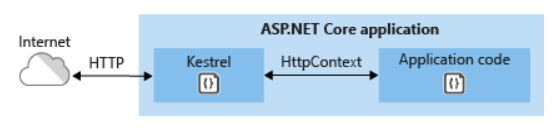
\includegraphics[width=17cm]{imgs/asp_structure.jpg}
\end{center}\vspace{-0.3cm}
\caption[ASP.NET Structure]{ASP.NET Structure} \label{asp_structure}
\end{figure}


The architectural framework is divided into four basic tiers: front-end, back-end, database, and file storage.

\begin{enumerate}
\item \textbf{Front-End}: the front end is user interface where the user completes a series of operations to control the application which is supported by HTTP request and HTTP response. It contains HTML code, JavaScript, JQuery and CSS)

\item \textbf{Back-End} when a static HTTP response is received from the web browser, ASP.NET Core will create an HttpRequest object that contains the request data, and invoke the correspondent view to handle this object. After the handle process, it will create and return a new HttpResponse object to the front-end view.
\item \textbf{Database}: ASP.NET Core controls the MySQL relational database which is hosted in Azure.
\item \textbf{File Storage}: The files selected by the user are uploaded to Azure Blob Storage.


\end{enumerate}

\begin{figure}[h]
\begin{center}
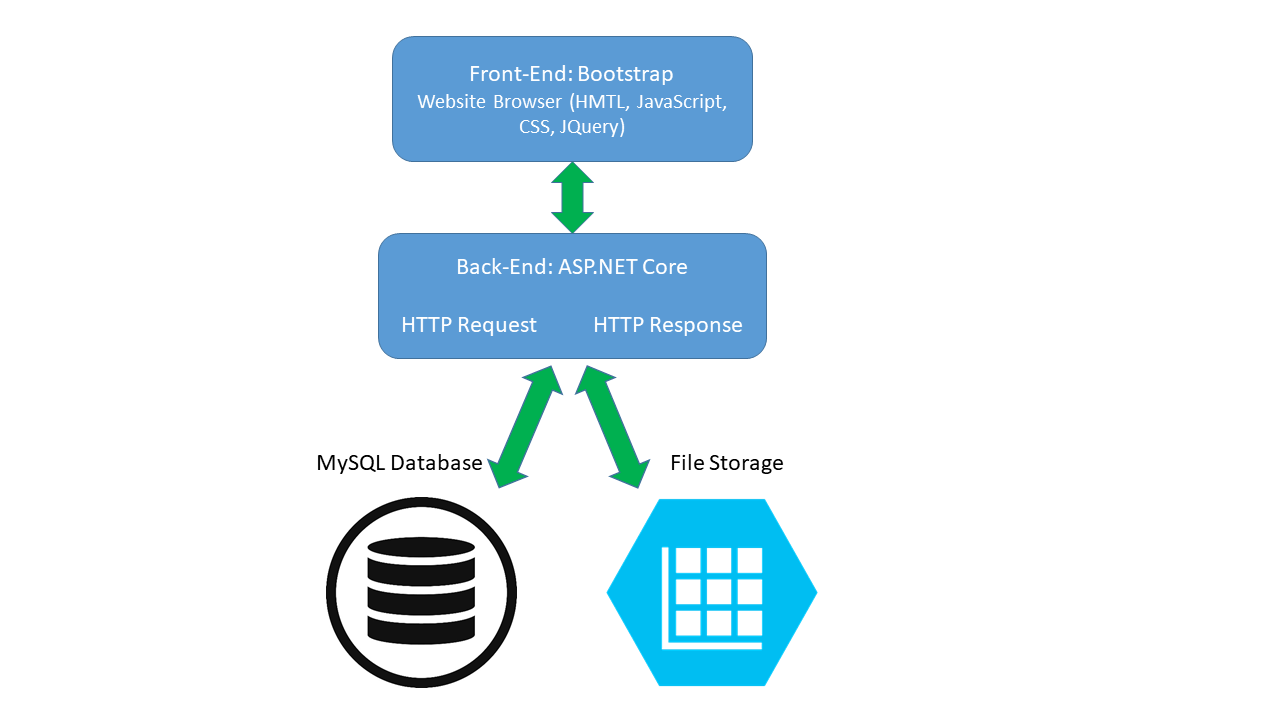
\includegraphics[width=17cm]{imgs/Application_Structure.png}
\end{center}\vspace{-0.3cm}
\caption[Application General Structure]{Application General Structure} \label{app_Structure}
\end{figure}


\section{Model-View-Controller Pattern}
\label{sub:MVC}

Due to the time limitations of the project the lack of experience in web designing, it was more appropriate to create a basic user interface and the devote the majority of the time to developing a robust back-end. Therefore, it was very important that the architecture of the application made a separation between the user interface and the back-end processing.

MVC framework is a one of the most popular design patterns which is motivated by the separation of the  UI and the processing performed to generate it. The MVC has been conceptualised for many years, and thus it precedes the inception of web applications and therefore, many efforts at applying the model to web applications through frameworks have been controversial.

Since most of the time has been devoted into developing the back-end than the front-end of the application, it is quite likely that at some point in the future the front-end would be replaced with a more aesthetically pleasing one.


The Model-View-Controller (MVC) architectural pattern separates an application into three main groups of components: Models, Views, and Controllers. This pattern helps to achieve separation of concerns. Using this pattern, user requests are routed to a Controller which is responsible for working with the Model to perform user actions and/or retrieve results of queries. The Controller chooses the View to display to the user, and provides it with any Model data it requires \cite{mvc}.


\begin{figure}[h]
\begin{center}
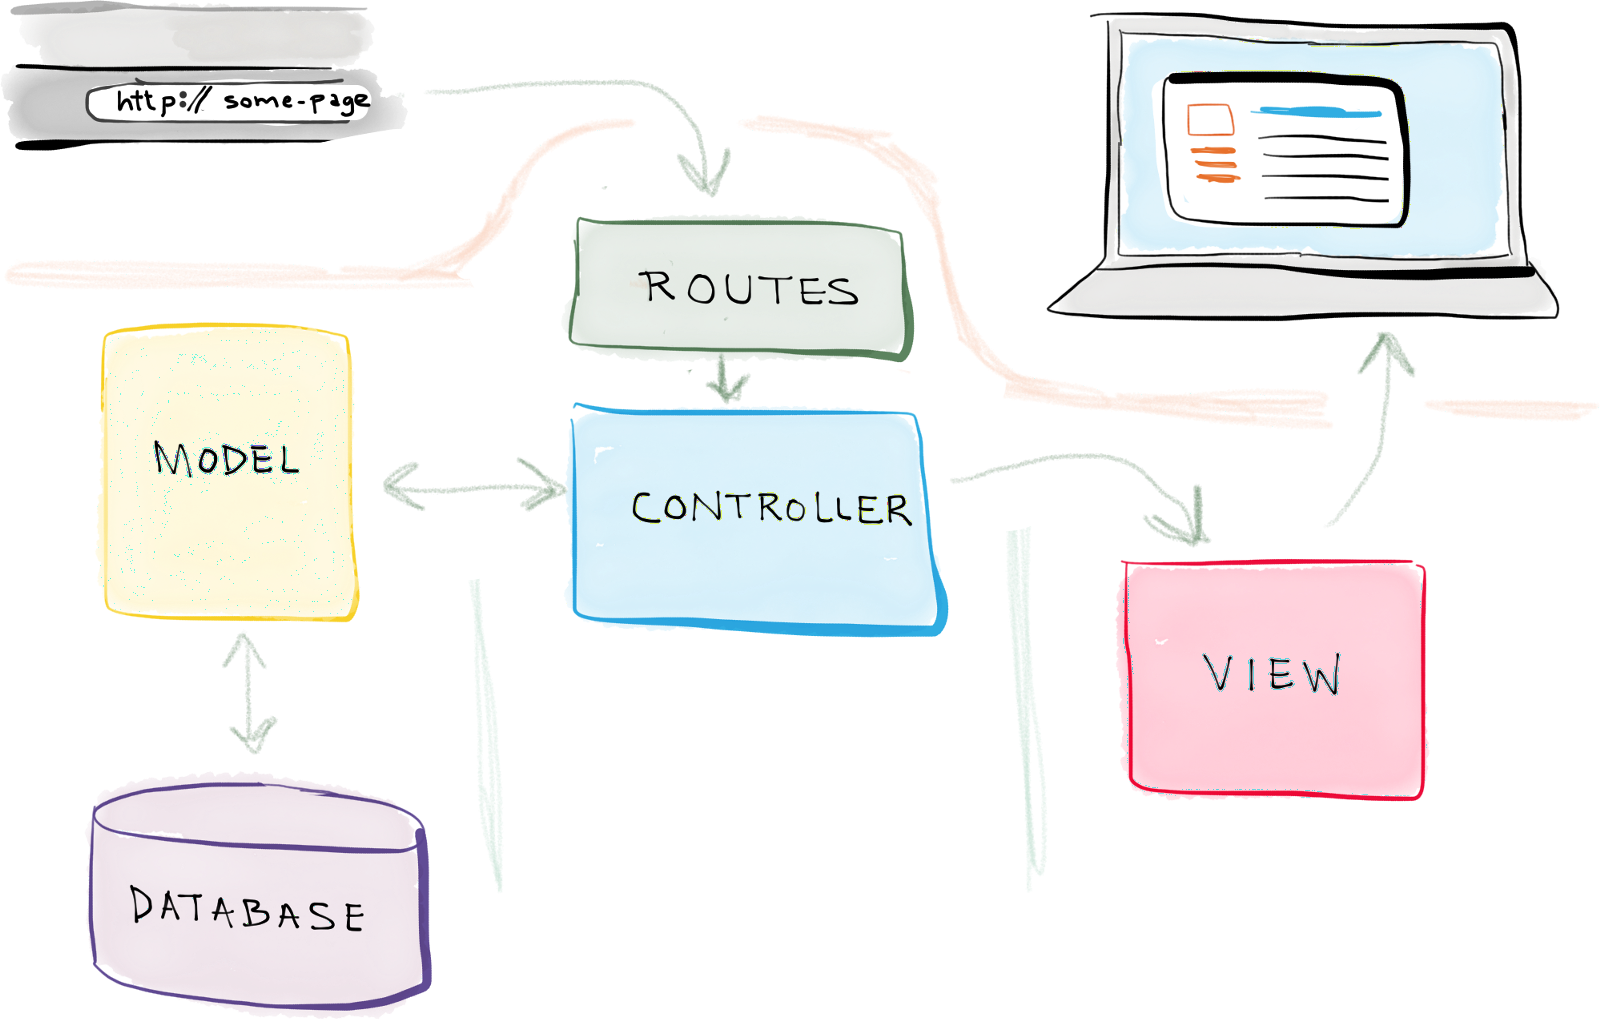
\includegraphics[width=17cm]{imgs/mvc.png}
\end{center}\vspace{-0.3cm}
\caption[The Model-View-Controller Pattern of ASP.NET Core]{The Model-View-Controller Pattern of ASP.NET Core} \label{mvc}
\end{figure}




\section{Design Class Diagram}
\label{sub:design_class_diagram}
 
\section{Database Design and ERD}
\label{sub:database_design_and_erd}


